\chapter{Background}

\section{Wireless Communication}
\section{\acf{LoRa}}


\section{\acf{LoRaWAN}}

% TODO network structure

\ac{LoRaWAN} data rates typically range from 0.3 kbps to 50 kbps, depending on the region and the \ac{LoRa} modulation used~\cite[p. 8]{lora_alliance_inc_lorawan_2017}.

\begin{figure}[ht]
    \centering
    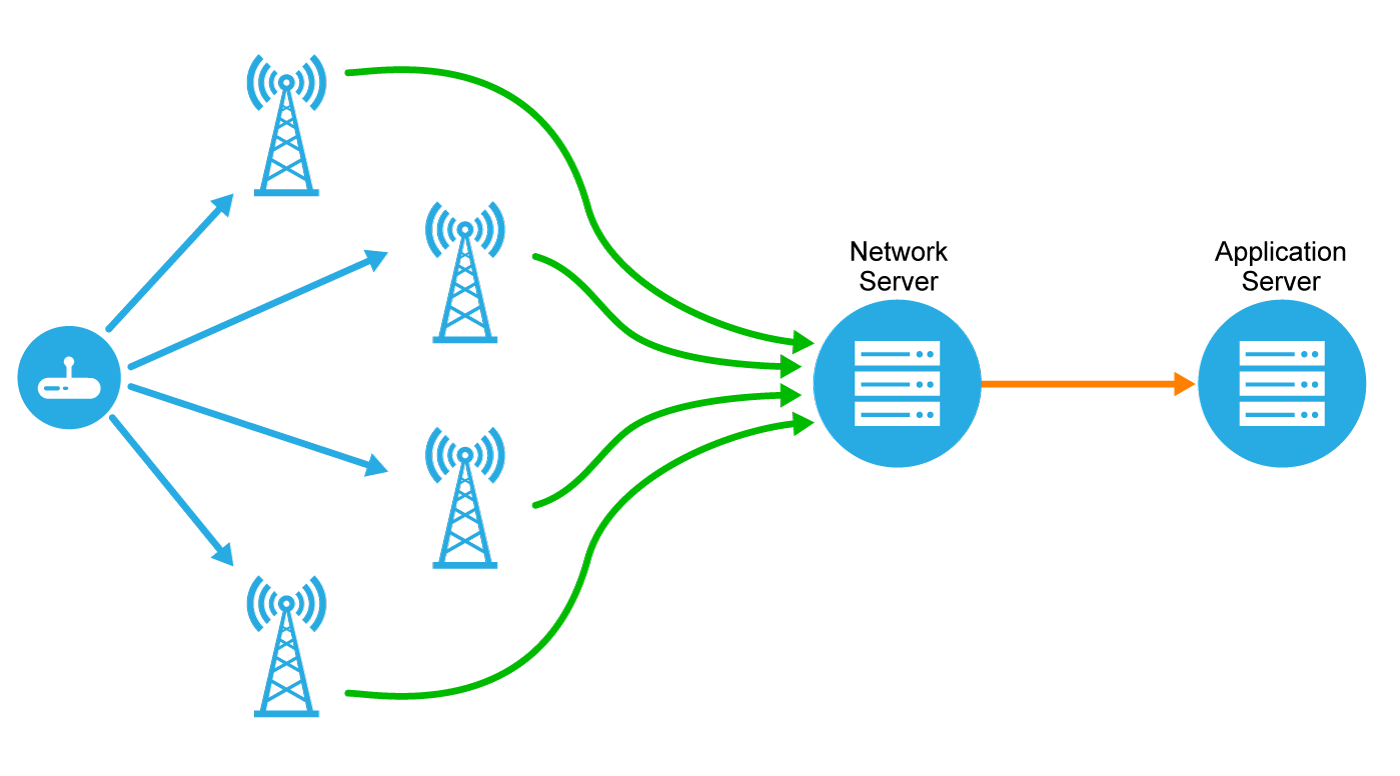
\includegraphics[width=0.9\textwidth]{pictures/lorawan-structure/topology_semtech_developers.png}
    \caption{\ac{LoRaWAN} network structure~\protect\cite{semtech_lora_developer_portal_-depth_nodate}}
    \label{pic:lorawan-network-structure}
\end{figure}

% TODO: explain what uplink and downlink are

\subsection{Device Classes}

\ac{LoRaWAN} defines three classes of devices that offer different variations of the trade-off between power consumption and data rate/availability~\cite[p. 10]{lora_alliance_inc_lorawan_2017}.

\subsubsection{Class A}

Class A is used for devices that need to consume as little power as possible.
Every \ac{LoRaWAN} device must support the Class A mode~\cite[p. 11]{lora_alliance_inc_lorawan_2017}.
A communication in Class A is always initiated by the end device itself.

Bidirectional communication is possible in Class A through the use of two downlink receive windows during which it is possible for the \ac{LNS} to send data to the device.
This also makes it impossible for the \ac{LNS} to send data to the device at any other time.

Class A consumes the least amount of power of the three classes, since the devices itself may specify when and how often they want to communicate with the \ac{LNS}.

\subsubsection{Class B}

In addition to class A, class B devices are also able to receive downlink messages from the \ac{LNS} during dedicated downlink receive windows.
In order to realize this without the need for a per-device RTC clock, class B devices receive time synchronized beacons from the gateways.

These scheduled downlink windows result in a higher power consumption for the devices, since they need to be awake during these windows.

\subsubsection{Class C}

Class C devices, when not currently transmitting an uplink message, are always listening for downlink messages from the \ac{LNS}.
In essence, they keep the downlink windows as specified in class B open all the time.

\subsection{Duty Cycle}

% TODO add a figure with the duty cycle

In the \ac{EU} region, the transmission duty cycle of devices in the 868 MHz band is limited to 1\%~\cite{etsi_etsi_2012}.
This means that a \ac{LoRa} device using this frequency may only transmit for 1\% of a given time slot.
It needs to stay silent for the rest of the time.

\section{\acf{LoRaWAN}}

\ac{LoRaWAN} uses the LoRa wireless communication protocol to create a \ac{WAN} where multiple devices can communicate with each other over long distances.

\subsection{\acf{TTN}}

\ac{TTN} provides a free to use \ac{LNS} that supports a global community of people building \ac{LoRaWAN} applications.
It provides a free \ac{LoRaWAN} network for the public to use.

\ac{TTN} was used in this thesis to enable the communication between the \ac{LoRa} devices and TTNMapper.

% TODO: Explain the CUPS and LNS architecture

\section{Localization}

\subsection{Technologies}

\subsubsection{\ac{GPS}}

% Genauigkeit von GPS mit quelle
% GPS verwendet lateration -> quelle

\subsection{Triangulation}

\subsection{Multilateration}

\subsection{\acs{ToA}-based}

The \acf{ToA} based method uses the difference in the signal's time of arrival at the receiving stations.
In conjunction with the speed of light, this time difference can be used to calculate the distance between the receiving stations and the transmitting station.

\ac{ToA} is being used by radio location systems like \ac{GPS} to determine the position of a device by using Multilateration.

\subsection{\acs{TDoA}-based}



\subsection{\acs{RSSI}-based}

The method based on \acf{RSSI} uses the signal strength of the signal that is received.
Since signal strengths are not linear, the \ac{RSSI} values need to be converted to a linear scale.
Different devices can have different \ac{RSSI} values for the same distance.
\ac{RSSI} values can only function reliably when there is nothing blocking the signal between the transmitting and receiving stations, e.g. if there is a line of sight between the sender and receiver.

\section{\ac{LoRa} Hardware}

\subsection{Gateways}

A \ac{LoRa} gateway is the device that receives \ac{LoRa} packets from \ac{LoRa} nodes and forwards them to the \ac{LoRaWAN} server.
Gateways are connected to the internet and can forward \ac{LoRaWAN} packets that it receives to the \ac{LNS} in two major ways:

\subsubsection{Semtech \acs{UDP} Packet Forwarder}

% TTN rät seit v3 davon ab

\subsubsection{\acf{TCP} / LoRa Basics\texttrademark~Station}

% Recommended by TTN

\subsection{Nodes}